\question{1.15}{Bij een verkeerscontrole zijn de banden van 200 auto's gecontroleerd. Hierbij werd het profiel gemeten in mm.
Een en ander leidde tot de volgende frequentieverdeling (zie de tabel).
    
    \begin{center}
        \begin{tabular}{lc}
            \toprule
            \textbf{Gemeten profiel (in mm)} & \textbf{Aantal auto's} \\
            \midrule
            $0{,}00-<2{,}00$ & 4 \\
            $2{,}00-<4{,}00$ & 34 \\
            $4{,}00-<6{,}00$ & 82 \\
            $6{,}00-<8{,}00$ & 66 \\
            $8{,}00-<10{,}00$ & 14 \\
            \midrule
            \textbf{Totaal} & 200 \\
            \bottomrule
        \end{tabular}
    \end{center}
}

\begin{enumerate}[label=(\alph*)]
    \item Geef de waargenomen verdeling weer door middel van een cumulatieve frequentiecurve.
    \answer{
        De cumulatieve frequentieverdeling is als volgt:
        \begin{center}
            \begin{tabular}{lcc}
                \toprule
                \textbf{Gemeten profiel (in mm)} & \textbf{Cumulatief aantal auto's} \\
                \midrule
                $0{,}00-<2{,}00$ & 4 \\
                $2{,}00-<4{,}00$ & 38 \\
                $4{,}00-<6{,}00$ & 120 \\
                $6{,}00-<8{,}00$ & 186 \\
                $8{,}00-<10{,}00$ & 200 \\
                \midrule
                \textbf{Totaal} & 200 \\
                \bottomrule
            \end{tabular}
        \end{center}

        De cumulatieve frequentiecurve ziet er als volgt uit:

        \begin{center}
            \resizebox{0.9\textwidth}{!}{
                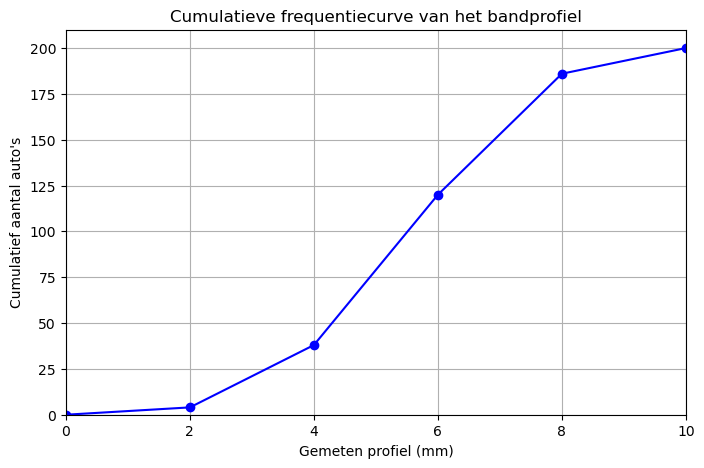
\includegraphics{opg1.15a.png}
            }
        \end{center}
    }
    
    \item Probeer met de grafiek te schatten hoe groot het aantal auto's is met een profiel van minder dan 5,00 mm.
    (NB In deze opgave mag men veronderstellen dat de klassengrenzen exact zijn, dus er hoeven geen correcties met 'halfjes' uitgevoerd te worden.)
    \answer{
        De schatting voor het aantal auto's metg hoogstens een profiel van 5,00mm vinden we
        door te interpoleren op de cumulatieve frequentiecurve van opgave (a).
        Dit ziet er als volgt uit:

        \begin{center}
            \resizebox{0.9\textwidth}{!}{
                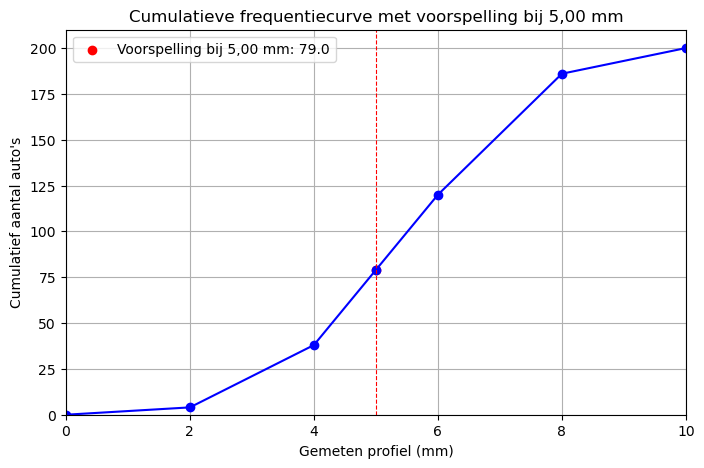
\includegraphics{opg1.15b.png}
            }
        \end{center}

        Naar schatting zullen er dus 79 auto's zijn met een profiel van hoogstens 5,00mm dikte.
    }
\end{enumerate}